\question \textbf{The Viterbi algorithm}

The Viterbi algorithm is a dynamic programming based method to find the optimal path of an HMM with hidden status.

\begin{figure}[H]
      \centering
      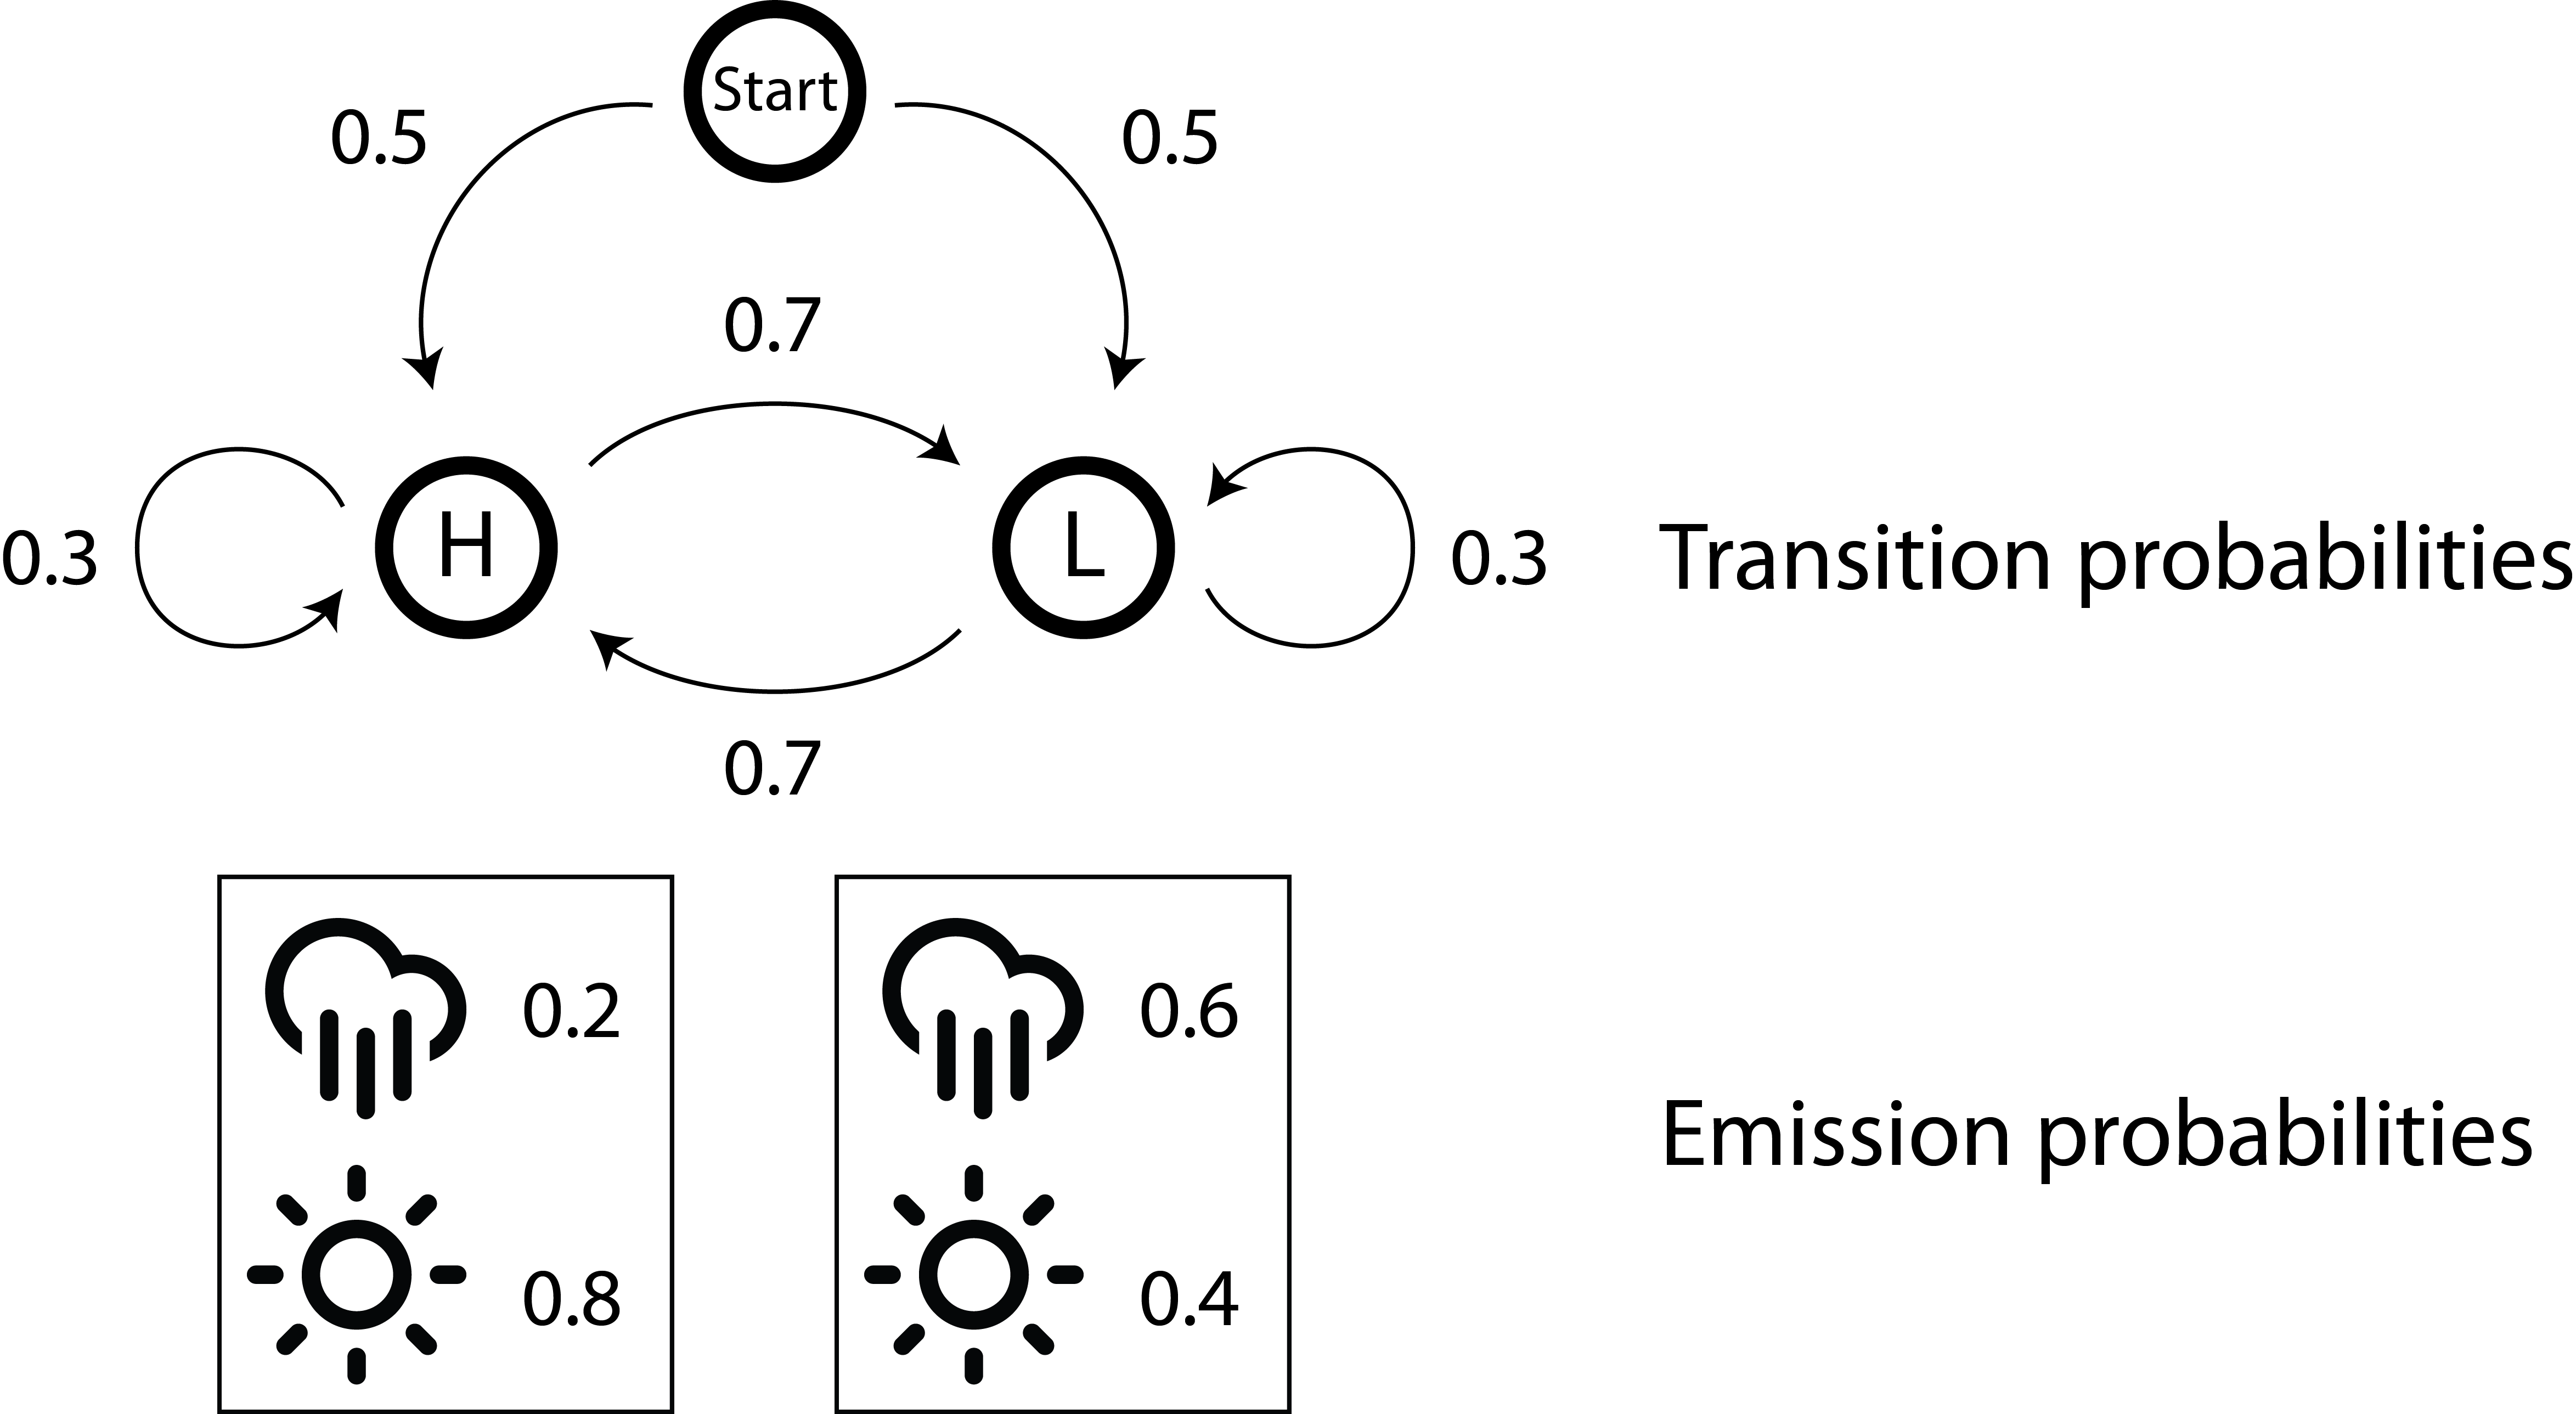
\includegraphics[width=0.6 \textwidth]{fig13/hmm_viterbi.png}
\end{figure}

\vspace{0.1 in}

\begin{parts}

%% (a)
  \part Find the optimal path when observed weather conditions are (Rain, Sunny).
\begin{table}[H]
\centering
\begin{tabular}{|c|c|c|}
\hline
      & H & L \\ \hline
Rain  &  \qquad  \qquad  \qquad  \qquad  \qquad \qquad  \qquad & \qquad  \qquad  \qquad \qquad  \qquad \qquad  \qquad \\ \hline
Sunny &   &   \\ \hline
\end{tabular}
\end{table}

\begin{solution}[0.35 in]
(L, H)
\end{solution}

%% (b)
  \part Find the optimal path when observed weather conditions are (Sunny, Sunny, Rain).
\begin{table}[H]
\centering
\begin{tabular}{|c|c|c|}
\hline
                           & H                     & L                     \\ \hline
Sunny  &  \qquad  \qquad  \qquad  \qquad  \qquad \qquad  \qquad & \qquad  \qquad  \qquad \qquad  \qquad \qquad  \qquad \\ \hline
Sunny   &                       &                       \\ \hline
Rain &  & \\ \hline
\end{tabular}
\end{table}

\begin{solution}[0.35 in]
(L, H, L)
\end{solution}

\end{parts}
